
\chapter{STABILITY AND RECONSTRUCTIONS OF PT/PD BIMETALLIC NANOCUBES EXPOSED TO CARBON MONOXIDE}

\section{Introduction}

Metals are used as catalysts in various industrial processes and because of the
importance of maximizing reactions ({\em i.e.} surface area to volume ratio),
many of these processes make use of roughened surfaces or nanoparticles
dispersed on a cheaper unreactive surface.\citep{Munnik:2015qf, Graham:2007ng}
The size distribution of nanoparticles tends to be on the order of tens to
hundreds of nanometers in size, which results in efficient utilization of the
material compared to a flat surface.\citep{Zhang:2011ne, Liu:2013hf}
Additionally, the morphology of these nanoparticles plays a role in their
activity and includes simple cubes, octahedra, pyramids, and numerous other
morphologies.\citep{Ahmadi:2015os, Wang:2015qb, Wang:2016dg} The different
morphologies can be somewhat characterized by their displayed stable facets;
however, as seen in previous work\citep{Tao:2010aa, Michalka:2013aa,
Michalka:2015aa, Kim:2016cr}, even fairly stable surfaces can undergo large
scale reconstructions under experimental conditions. This appendix provides
information on the initial setup of bimetallic Pt/Pd nanocubes and the
preliminary results obtained. 

\section{Methodology}
\subsection{Interaction Potentials}
The interaction potentials provided in Michalka {\em et
al.}\citep{Michalka:2015aa} are used here unchanged. It is important to note
that with the potential the \ce{Pd\bond{-}CO} binding interaction is 0.2
kcal/mole more favorable than the \ce{Pt\bond{-}CO} interaction. Additionally,
the treatment of the metal interactions results in \ce{Pt\bond{-}Pt} bonds
being stronger than \ce{Pt\bond{-}Pd} bonds, which are stronger than
\ce{Pd\bond{-}Pd} bonds.

\subsection{System details}
Nanocubes with edge lengths of 6, 7, and 8 nm were constructed from an ideal
\ce{Pd} FCC lattice with a lattice constant of 3.89 \AA~  and cut so as to
expose the (100), (010), and (001) facets. For each of these three sizes, the
outermost 1, 2, or 3 layers were further replaced with Pt to create nine total
systems whose compositions are reported in Table \ref{tab:systems}. Work by Cao
{\it et al.}\citep{Cao:2010gf} on the self-distillation of bimetallic
nanostructures (\ce{Rh/Pt}) showed that when the outer shell of the particle
was composed of the higher melting metal (\ce{Rh}) there was an imposed stability on the
confined inner metal (\ce{Pt}). For our systems, \ce{Pt} ($T_m = 2041 K$) is the higher melting
metal and was chosen to compose the outer layers while keeping the core of the
nanoparticle Pd ($T_m = 1828 K$). 

%Additionally, the slightly more favorable Pd-CO interaction may provide a driving force for reconstructions that will be dependent on the thickness of the Pt since Pd will want to migrate through the Pt to the surface.

\begin{table}
  \caption{PT/PD NANOCUBE SIZES AND COMPOSITION}
  \centering
  \begin{threeparttable}
  \begin{tabular}{ c ccc }
  \hline
  \hline
  \textbf{System} & \textbf{Pd} & \textbf{Pt} &  \textbf{(Pt/total)} \\
  \hline
  6nm-1L & 10976 & 2524  & 0.187 \\
  6nm-2L & 8788  & 4712  & 0.349 \\
  6nm-3L & 6912  & 6588  & 0.488 \\
  7nm-1L & 19652 & 3676  & 0.157 \\
  7nm-2L & 16384 & 6944  & 0.298 \\
  7nm-3L & 13500 & 9828  & 0.421 \\
  8nm-1L & 27436 & 4564  & 0.143 \\
  8nm-2L & 23328 & 8672  & 0.271 \\
  8nm-3L & 19652 & 12348 & 0.386 \\
  \hline
  \hline
  \end{tabular}
  \end{threeparttable}
\label{tab:systems}
\end{table}

Systems were constructed in a orthorhombic periodic box of greater size that
the nanocubes that were contained within. The systems were then initially
equilibrated at 5~K to allow the slight strain of replacing Pd atoms with Pt in
the outer layers to dissipate while maintaining the nanocube morphology.
Warming over approximately 3~ns was performed to bring all systems up to a
simulation temperature of 1000~K at which point an amount of CO equivalent to a
0.5 ML coverage was introduced into the system.  After another brief period of
equilibration during which a significant amount of the CO adsorbed to the
surface, the systems were run for an additional 3~ns of
data collection.

Figures \ref{fig:6nm}, \ref{fig:7nm}, and \ref{fig:8nm} highlight the different
nanocube systems after the initial strain relaxation and then after the systems
have been warmed but before the CO was added. The instability of the smaller
systems as highlighted in Figures \ref{fig:6nm}, \ref{fig:7nm}.a, and
\ref{fig:8nm}.a is one the reasons this project was paused.  Specifically, the
6 nm systems underwent extreme distortions from the nanocube morphology during
the warming procedure and even at 750~K (before warming was complete) as
displayed in the image, the original (100) surface has almost entirely been
replaced with the more stable (111) surface. The larger mass of the 7 and 8 nm
systems allowed for a greater amount of stability; however, the 1L systems for
both sizes still experienced an extremely large amount of non \ce{CO}-induced
restructuring.

\begin{landscape}
\begin{figure}[p!]
\centering
  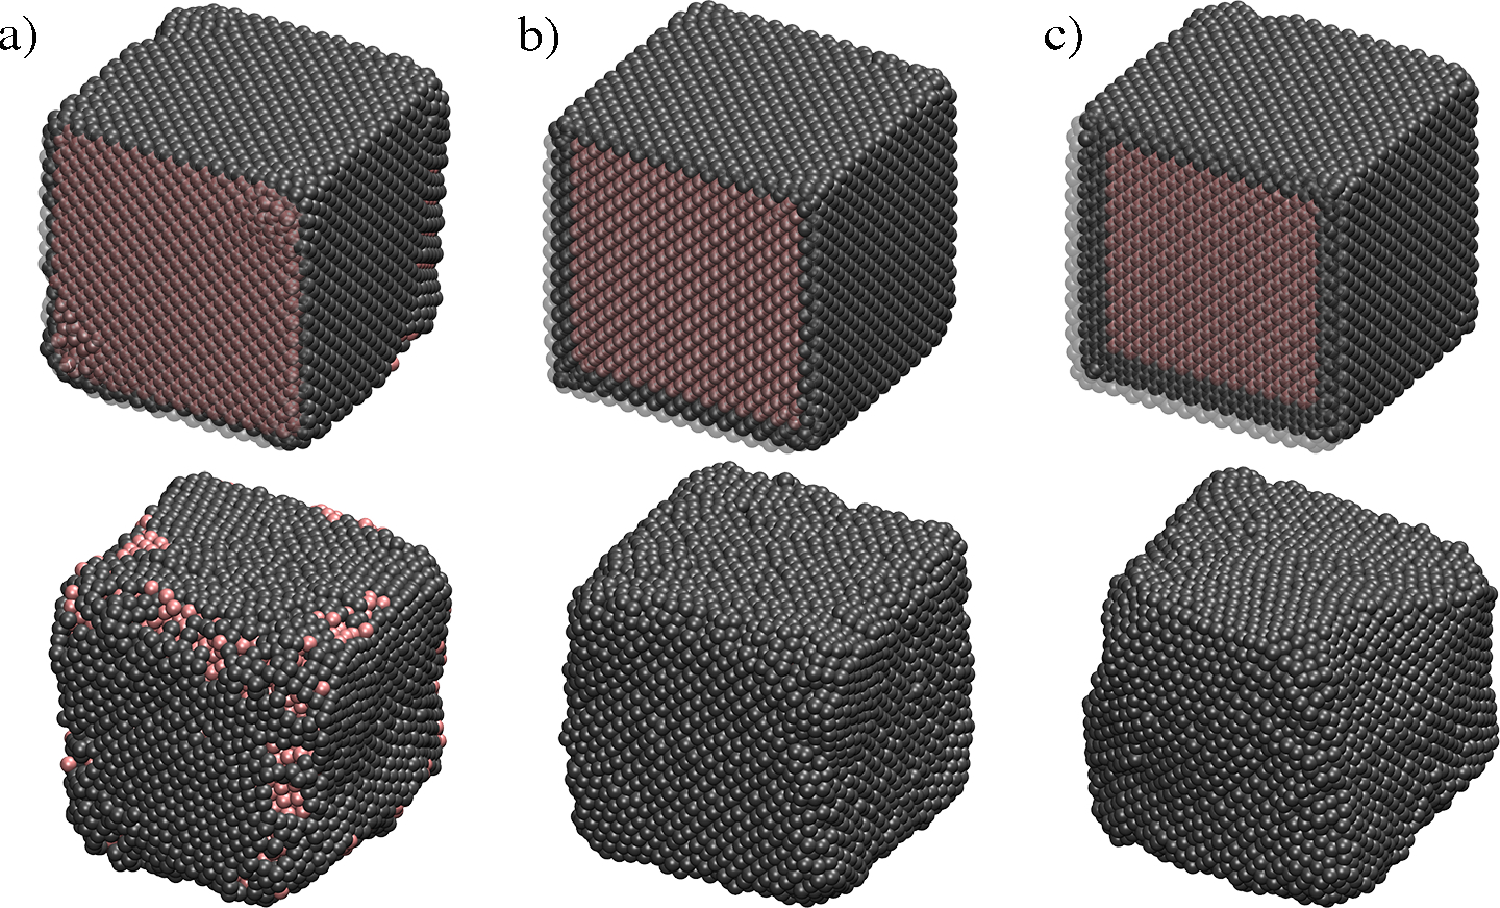
\includegraphics[width=0.8\linewidth]{../figures/appB/6nm.pdf}
  \caption{The top row displays the 6 nm nanocubes at 300~K in the midst of the
warming procedure.  \ce{Pt} atoms are shown in gray while \ce{Pd} atoms are
shown in pink.  There is a slight transparency of the front \ce{Pt} face to
show the inner \ce{Pd} atoms. The bottom row depicts the same systems after
warming to 750~K.  (a) corresponds to the one-layer (1L) system while (b) and
(c) correspond to the 2L and 3L systems respectively.}
  \label{fig:6nm}
\end{figure}
\end{landscape}

\begin{landscape}
\begin{figure}[p!]
\centering
  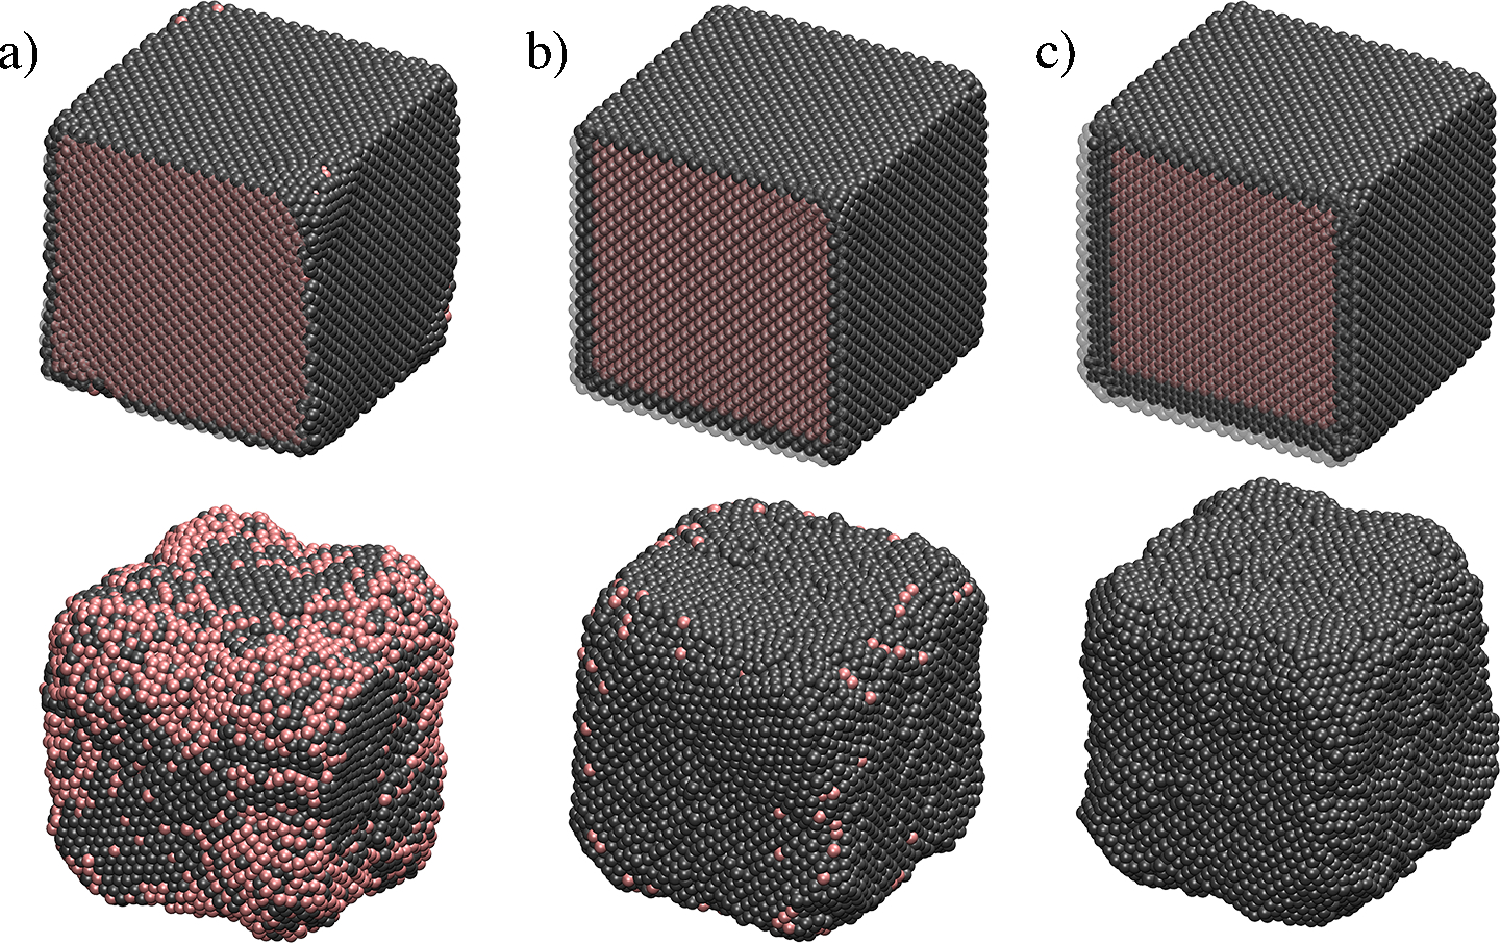
\includegraphics[width=0.8\linewidth]{../figures/appB/7nm.pdf}
  \caption{The top row displays the 7 nm nanocubes at 300~K in the midst of the warming procedure.
The bottom row depicts the same systems after warming to
1000~K.  (a) corresponds to the one-layer (1L) system while (b) and (c)
correspond to the 2L and 3L systems respectively. The 7nm-1L system is somewhat
unstable and shows significant deviations away from the original (100) facets.}
  \label{fig:7nm}
\end{figure}
\end{landscape}

\begin{landscape}
\begin{figure}[p!]
\centering
  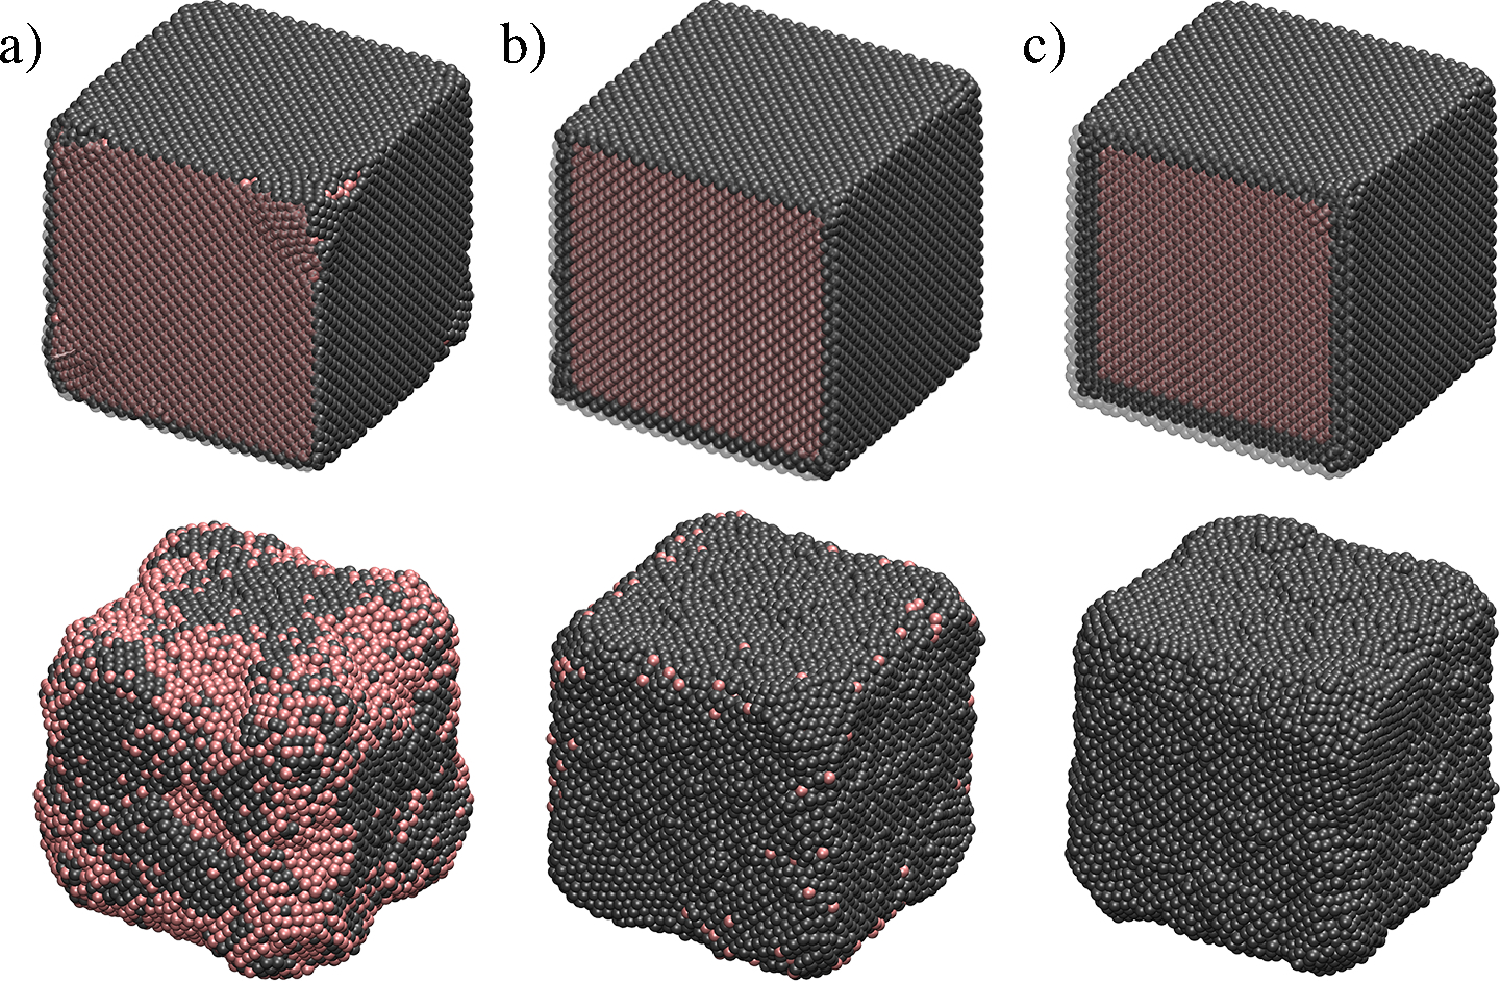
\includegraphics[width=0.8\linewidth]{../figures/appB/8nm.pdf}
  \caption{The top row displays the 8 nm nanocubes after at 300~K in the midst of the warming procedure. 
The bottom row depicts the same systems after warming to
1000~K.  (a) corresponds to the one-layer (1L) system while (b) and (c)
correspond to the 2L and 3L systems respectively. Similar to the 7nm-1L system,
the 8nm-1L nanocube undergoes significant restructuring to maximize the
formation of (111) domains on the surface.}
  \label{fig:8nm}
\end{figure}
\end{landscape}



\section{Results \& Discussion}
One of the challenges that led to this project being shelved is the size of the
systems and the concomitant increase in simulation time needed to capture the
hypothesized restructuring processes. The 3 nanoseconds that were simulated
provided us with the following results which are discussed below.


\subsection{CO-Induced reconstruction}
As concluded in our previous work\citep{Michalka:2013aa}, the presence of CO was again
seen to play a role in the observed restructuring. However, unlike what was
observed on the \ce{Pt} (557) surface, where \ce{CO} was
required for any large-scale reconstruction to occur, for these systems a
significant portion of the reconstruction could be directly attributed to the lower
stability of the (100) facets when compared to (111) facets. As highlighted in
Figure \ref{fig:6nm}, these systems underwent an extreme amount of
reconstruction despite no \ce{CO} being present. 

However, Figure \ref{fig:8nmCO}.b does show that the more favorable
\ce{Pd\bond{-}CO} binding does lead to an inversion or surface segregation of
the inner Pd to the surface of the nanocube. \ce{Pd} was preferentially found
to have segregated to the surface near the edges and corners of the cubes which
is easily explained as the surface atoms at those sites tend to be
undercoordinated and thus are easier to break their surface bonds.

Surface energy arguments can also be made to explain some of the restructuring.
As mentioned in the system details, the EAM forcefield that is being used to
describe the metal-metal interactions results in a Pt-Pd bond that is more
favorable than a Pd-Pd bond.  Thus, given sufficient time and energy to
overcome kinetic barriers, all of the Pt on the surface would prefer to be
subsumed underneath the Pd. However, there is a competing process which could
cause surface \ce{Pt} to sinter so as to maximize Pt-Pt bonds. While this may
result in a lower overall energy for the system, the potential barrier is quite
high as there would have to be numerous ``lifting'' processes to build up the
multiple layers of \ce{Pt} needed to maximize the number of \ce{Pt\bond{-}Pt}
interactions. Additionally, this would expose a significant amount of the
buried \ce{Pd}, which will \ce{CO} would prefer this, it would also increase
the total surface area of the system which is an energetically unfavorable
process.


\begin{landscape}
\begin{figure}[p!]
\centering
  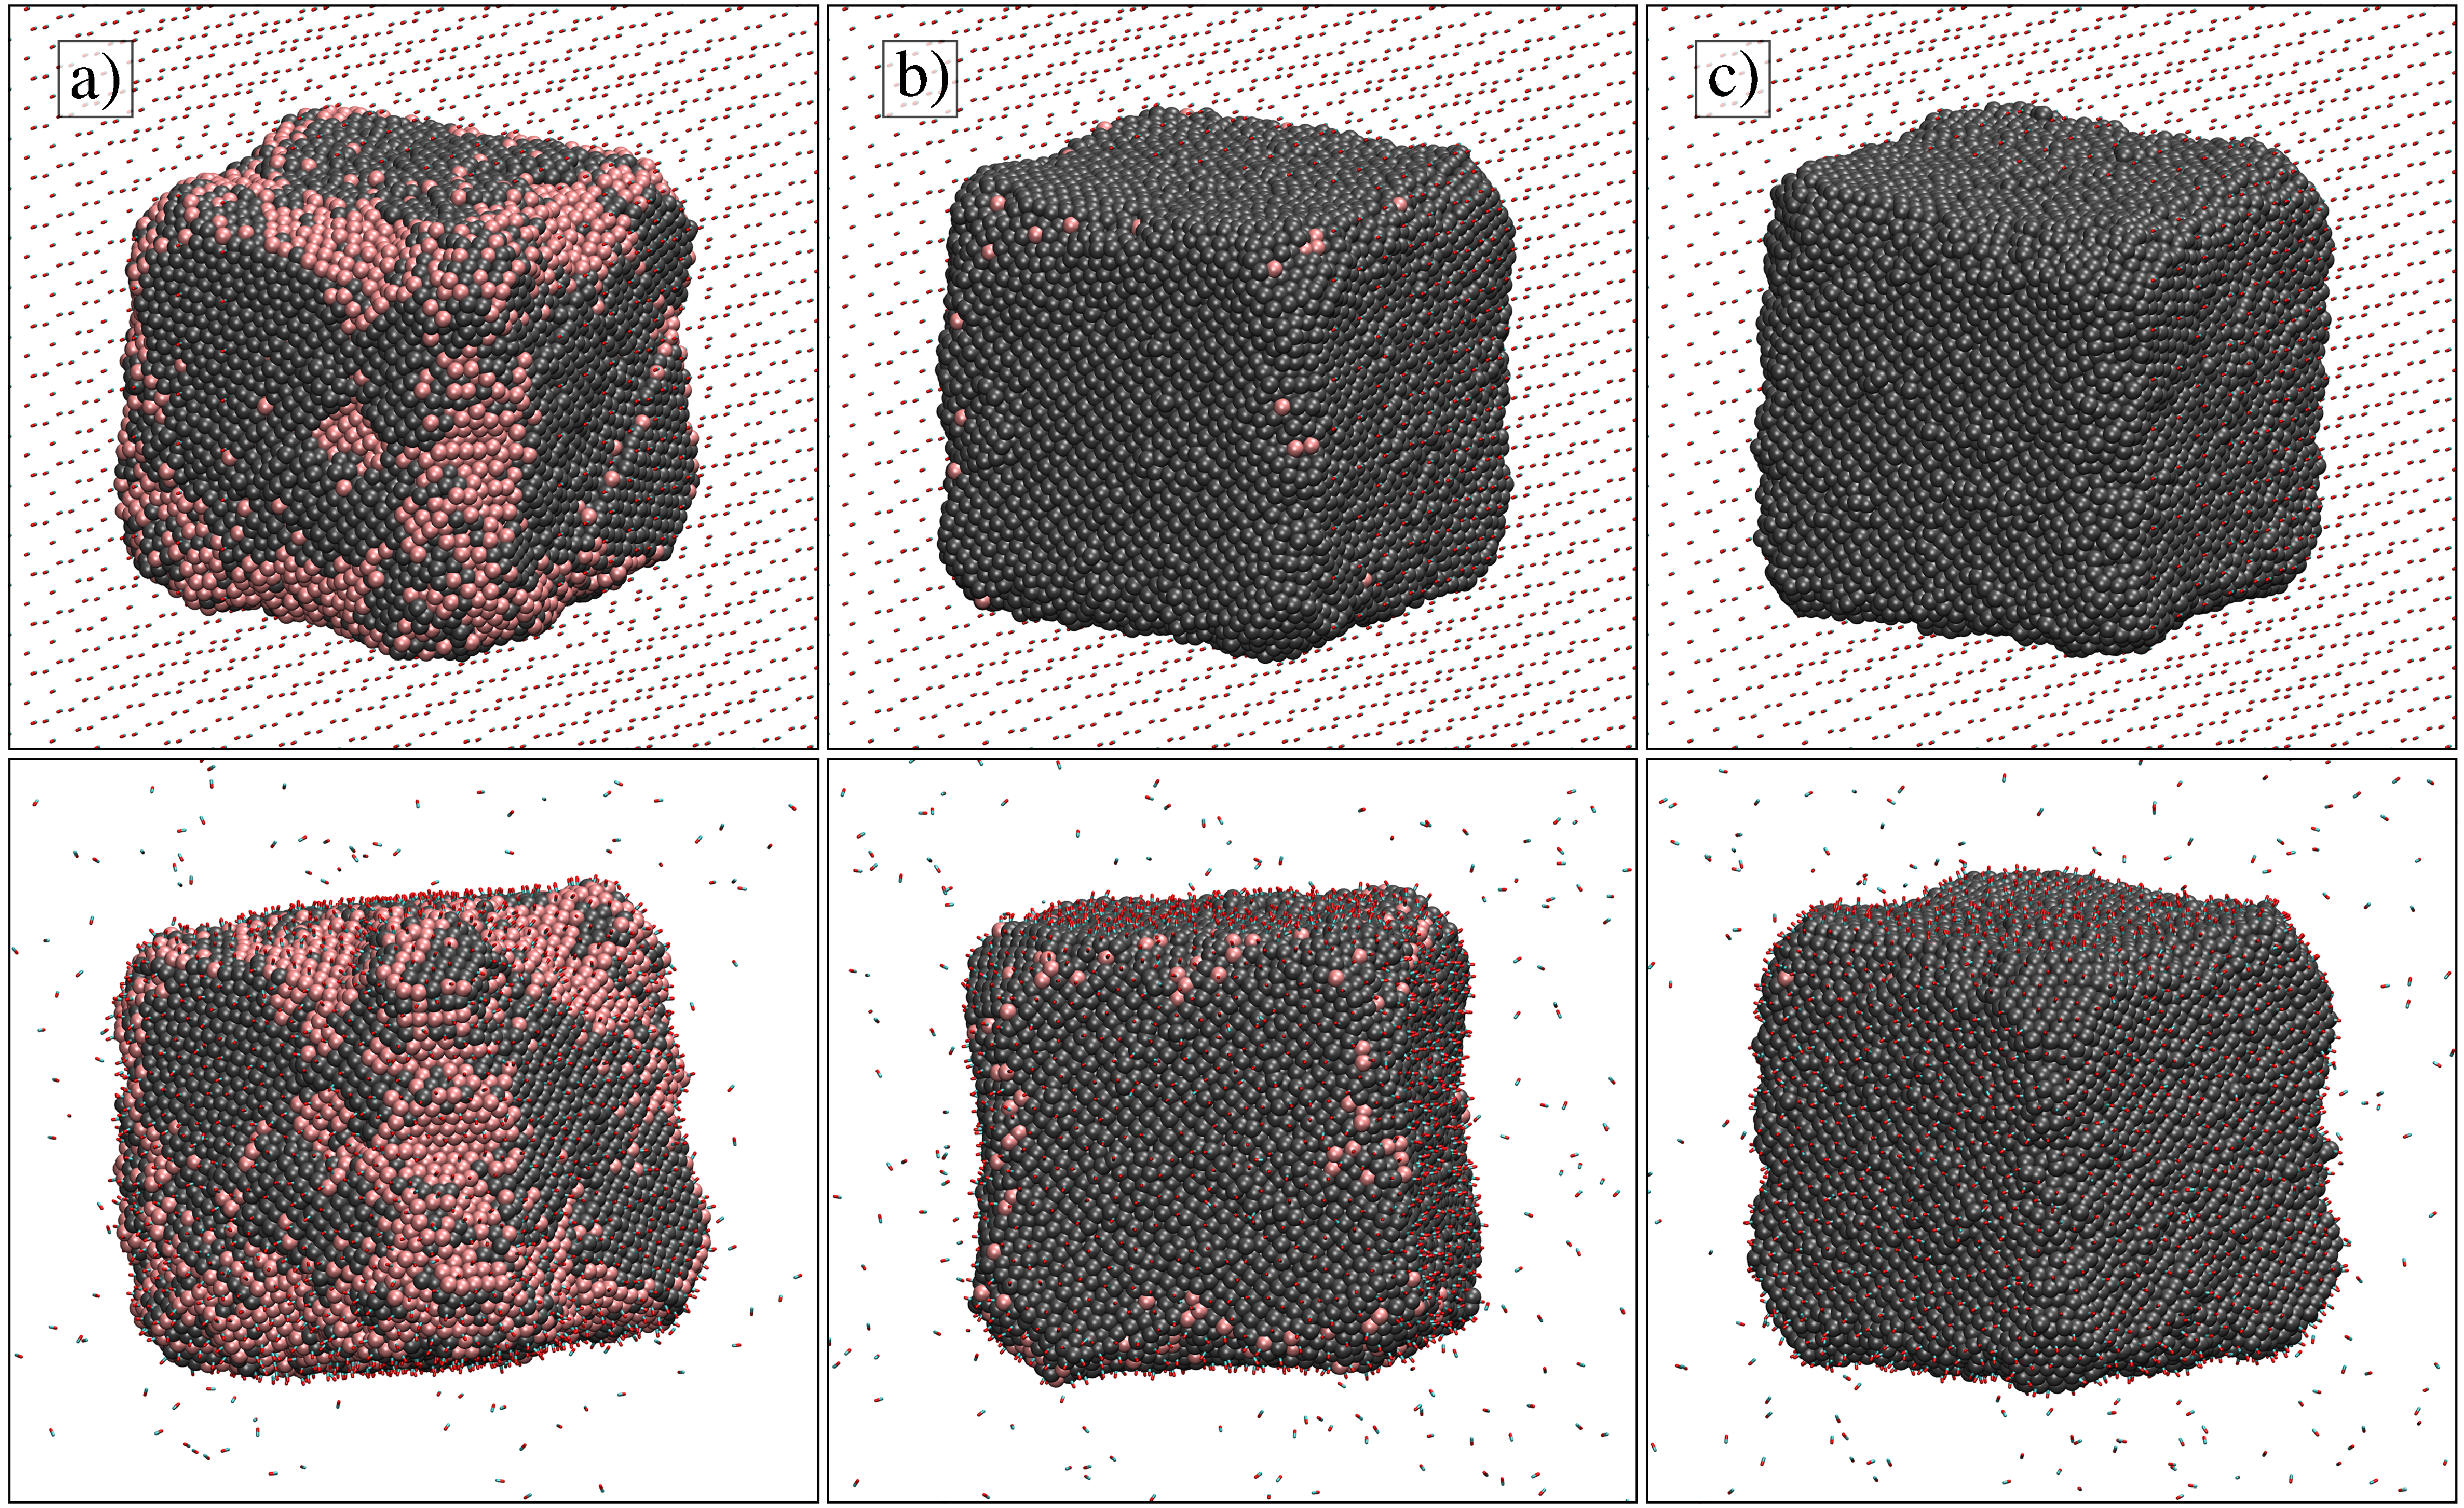
\includegraphics[width=0.8\linewidth]{../figures/appB/8nm_CO.pdf}
  \caption{The top row depicts the 8 nm nanocubes surrounded by the equivalent
of 0.5 ML of CO. The bottom row shows the same systems after 3 ns.  The small
amount of rotation is due to an improperly sampled velocity distribution of the
CO which upon adsorption and collision with the nanocube imparted a slight
rotation.}
  \label{fig:8nmCO}
\end{figure}
\end{landscape}



\section{Summary}
The observed restructuring while informative, was primarily determined to be an
artifact of the small system sizes that were chosen for this investigation.
Future simulations examining larger systems ($>10$ nm) may solve the buckling
observed in a number of these systems. Additionally, an exploration into
octahedral-type nanoparticles with their preferred (111) facets may also help
solve the stability issues and provide another direction to explore.
